\chapter{Convolutional Neural Network (CNN/ ConvNet) \cite{dnn-1,gfg-convolutional-neural-network-cnn-in-machine-learning}}\label{Convolutional Neural Network}

\begin{enumerate}
    \item Convolutional Neural Networks, or CNNs, are a specialized class of neural networks designed to effectively process grid-like data, such as images.

    \item A Convolutional Neural Network (CNN) is a type of deep learning algorithm that is particularly well-suited for image recognition and processing tasks.
\end{enumerate}




\section{Image Processing \cite{dnn-1}}

\begin{enumerate}
    \item Image data is represented as a two-dimensional grid of pixels, be the image monochromatic or in color.

    \item Accordingly each pixel corresponds to one or multiple numerical values respectively.

\end{enumerate}



\subsection{Channels \cite{dnn-1}}

\begin{enumerate}[itemsep=0.15cm]
    \item The convolutional layer picks windows of a given size and weighs intensities according to the filter $\mathsf{V}$

    \item images consist of three channels: red, green, and blue (RGB)

    \item images are not two-dimensional objects but rather third-order tensors, characterized by a height, width, and channel, e.g., with shape $1024 \times 1024 \times 3$ pixels.

    \item While the first two of these axes concern spatial relationships, the third can be regarded as assigning a multidimensional representation to each pixel location.

    \item[] 
    $
        \hfill
        \text{ input : } \mathsf{X} = (\mathsf{X})_{i,j,k}
        \hfill
        \text{ filter : } \mathsf{V} = (\mathsf{V})_{a,b,c}
        \hfill
    $

    \item We could think of the hidden representations as comprising a number of two-dimensional grids stacked on top of each other.\\
    As in the inputs, these are sometimes called \textbf{channels}.\\
    They are also sometimes called \textbf{feature maps}, as each provides a spatialized set of learned features for the subsequent layer.

    \item[] 
    $
        \hfill
        [\mathsf{H}]_{i,j,d} 
        = \dsum_{a = -\Delta}^{\Delta} 
            \dsum_{b = -\Delta}^{\Delta} 
            \dsum_c [\mathsf{V}]_{a, b, c, d} [\mathsf{X}]_{i+a, j+b, c}
        \hfill
    $\\[1ex]
    where $d$ indexes the output channels in the hidden representations $\mathsf{H}$

    \item The subsequent convolutional layer will go on to take a third-order tensor, $\mathsf{H}$, as input.

    
\end{enumerate}




\section{Invariance \cite{dnn-1}}

\begin{enumerate}
    \item In the earliest layers, our network should respond similarly to the same patch, regardless of where it appears in the image. This principle is called \textbf{translation invariance}\indexlabel{translation invariance} (or \textbf{translation equivariance}\indexlabel{translation equivariance}).

    \item The earliest layers of the network should focus on local regions, without regard for the contents of the image in distant regions. This is the \textbf{locality principle}\indexlabel{locality principle}.\\
    Eventually, these local representations can be aggregated to make predictions at the whole image level.

    \item As we proceed, deeper layers should be able to capture longer-range features of the image, in a way similar to higher level vision in nature.

\end{enumerate}



\section{Constraining the MLP \cite{dnn-1}}

\begin{customTableWrapper}{1.5}
\begin{table}[H]
    \centering
    \begin{tabular}{l p{8cm}}
        $\mathbf{X}$ & two-dimensional images \\
        $[\mathbf{X}]_{i, j}$ & pixel at location $(i,j)$ in the input image \\

        $\mathbf{H}$ & immediate hidden representations \\
        $[\mathbf{H}]_{i, j}$ & pixel at location $(i,j)$ in the hidden representation \\

        $\mathsf{W}$ & fourth-order weight tensors \\
        $\mathbf{U}$ & biases \\
    \end{tabular}
\end{table}
\end{customTableWrapper}


\begin{enumerate}[itemsep=0.2cm]
    \item both $\mathbf{X}$ and $\mathbf{H}$ have the same shape

    \item[] 
    $
        \hfill
        \begin{aligned} 
        \left[\mathbf{H}\right]_{i, j} 
        &= [\mathbf{U}]_{i, j} + \dsum_k \dsum_l[\mathsf{W}]_{i, j, k, l}  [\mathbf{X}]_{k, l}\\ 
        &=  [\mathbf{U}]_{i, j} + \dsum_a \dsum_b [\mathsf{V}]_{i, j, a, b}  [\mathbf{X}]_{i+a, j+b}
        \end{aligned}
        \hfill
    $

    \item The switch from $\mathsf{W}$ to $\mathsf{V}$ is entirely cosmetic for now since there is a one-to-one correspondence between coefficients in both fourth-order tensors.

    \item We simply re-index the subscripts $(k, l)$ such that $k = i+a$ and $l = j+b$.
    \[
        \hfill
        [\mathsf{V}]_{i, j, a, b} = [\mathsf{W}]_{i, j, i+a, j+b}
        \hfill
    \]

    \item The indices $a$ and $b$ run over both positive and negative \textbf{offsets}, covering the entire image.

    \item For any given location $(i, j)$ in the hidden representation $[\mathbf{H}]_{i, j}$, we compute its value by summing over pixels in $x$, centered around $(i, j)$ and weighted by $[\mathsf{V}]_{i, j, a, b}$.

\end{enumerate}

\subsection{Translation Invariance \cite{dnn-1}}

\begin{enumerate}[itemsep=0.2cm]
    \item This implies that a shift in the input $\mathbf{X}$ should simply lead to a shift in the hidden representation $\mathbf{H}$\\
    This is only possible if $\mathsf{V}$ and $\mathbf{U}$ do not actually depend on $(i, j)$.

    \item[] $[\mathsf{V}]_{i, j, a, b} = [\mathbf{V}]_{a, b}$ 
    \hfill and \hfill
    $\mathbf{U} = u = \text{ constant} \hfill$ 

    \item[] 
    $
        \hfill
        [\mathbf{H}]_{i, j} 
        = u + \dsum_a\dsum_b [\mathbf{V}]_{a, b}  [\mathbf{X}]_{i+a, j+b}
        \hfill
    $

    \item This is a \textbf{convolution}\\
    We are effectively weighting pixels at $(i+a, j+b)$ in the vicinity of location $(i, j)$ with coefficients $[\mathbf{V}]_{a, b}$ to obtain the value $[\mathbf{H}]_{i, j}$

    \item $[\mathbf{V}]_{a, b}$ needs many fewer coefficients than $[\mathsf{V}]_{i, j, a, b}$ since it no longer depends on the location within the image

\end{enumerate}


\subsection{Locality \cite{dnn-1}}

\begin{enumerate}[itemsep=0.2cm]
    \item we believe that we should not have to look very far away from location $(i,j)$ in order to glean relevant information to assess what is going on at $[\mathbf{H}]_{i, j}$

    \item This means that outside some range $|a|> \Delta$ or $|b|> \Delta$, we should set $[\mathbf{V}]_{a, b} = 0$

    \item[] 
    $
        [\mathbf{H}]_{i, j} = u + \dsum_{a = -\Delta}^{\Delta} \dsum_{b = -\Delta}^{\Delta} [\mathbf{V}]_{a, b}  [\mathbf{X}]_{i+a, j+b}
        \hfill
        \text{(aka convolutional layer/ cross-correlation)}
    $

    \item $\mathbf{V}$ is referred to as a \textbf{convolution kernel}\indexlabel{convolution kernel}, a \textbf{filter}, or simply the \textbf{layer’s weights} that are learnable parameters.

    \item The price paid for this drastic reduction in parameters is that our features are now translation invariant and that our layer can only incorporate local information, when determining the value of each hidden activation. 
    
    \item All learning depends on imposing inductive bias. 
    
    \item When that bias agrees with reality, we get sample-efficient models that generalize well to unseen data. 
    
    \item But of course, if those biases do not agree with reality, e.g., if images turned out not to be translation invariant, our models might struggle even to fit our training data.

    \item deeper layers should represent larger and more complex aspects of an image. This can be achieved by interleaving nonlinearities and convolutional layers repeatedly.
\end{enumerate}

SEE: \fullref{function: Convolution}






\section{Layers}
\subsection{Convolutional Layer}

SEE: \fullref{nn: Convolution Layer}


\subsection{Pooling Layer}

SEE: \fullref{nn: Pooling Layer}


\subsection{Fully Connected Layer/ Dense Layer}
SEE: \fullref{nn: Linear Layer/ Dense Layer}





\section{General Network Design \cite{gfg-convolutional-neural-network-cnn-in-machine-learning,dnn-1}}\label{cnn: General Network Design}

\begin{figure}[h]
    \centering
    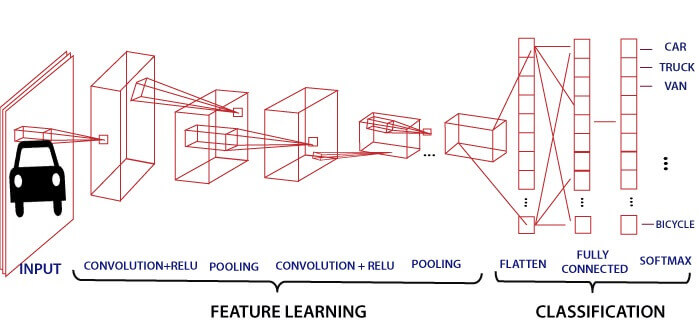
\includegraphics[width=\linewidth, height=5cm, keepaspectratio]{Pictures/convolutional-neural-network/convolutional-neural-network.jpg}
    \caption{CNN: General Network Design}
\end{figure}

\begin{enumerate}
    \item The construction of a convolutional neural network is a multi-layered feed-forward neural network, made by assembling many unseen layers on top of each other in a particular order.

    \item It is the sequential design that give permission to CNN to learn hierarchical attributes.
    
    \item In CNN, some of them followed by grouping layers and hidden layers are typically convolutional layers followed by activation layers.
    
    \item The pre-processing needed in a ConvNet is kindred to that of the related pattern of neurons in the human brain and was motivated by the organization of the \textbf{Visual Cortex}.

    \item  the most popular neural network architectures, we actually increase the channel dimension as we go deeper in the neural network, typically downsampling to trade off spatial resolution for greater \textbf{channel depth}.
\end{enumerate}






